% Customizable fields and text areas start with % >> below.
% Lines starting with the comment character (%) are normally removed before release outside the collaboration, but not those comments ending lines


%%%%%%%%%%%%% local definitions %%%%%%%%%%%%%%%%%%%%%
\newcommand{\mytitle}{PCC linearity studies with high pileup Run II data}
\newcommand{\instlumiunit}{$\times 10^{34} cm^{-2} s^{-1}$}
\newcommand{\zerobias}{$ZeroBias$}
\newcommand{\random}{$Random$}


%%%%%%%%%%%%%%%  Title page %%%%%%%%%%%%%%%%%%%%%%%%
\cmsNoteHeader{IN-XX-XXX} % This is over-written in the CMS environment: useful as preprint no. for export versions
% >> Title: please make sure that the non-TeX equivalent is in PDFTitle below for papers. For PASs, PDFTitle can be used with plain TeX.
\title{\mytitle}

% >> Authors
%Author is always "The CMS Collaboration" for PAS and papers, so author, etc, below will be ignored in those cases
%For multiple affiliations, create an address entry for the combination
%To mark authors as primary, use the \author* form
\address[inst1]{Universidad de Sonora}
\author*[inst1]{J. F. Benitez}

% >> Date
% The date is in yyyy/mm/dd format. Today has been
% redefined to match, but if the date needs to be fixed, please write it in this fashion.
\date{\today}

% >> Abstract
% Abstract processing:
% 1. **DO NOT use \include or \input** to include the abstract: our abstract extractor will not search through other files than this one.
% 2. **DO NOT use %**                  to comment out sections of the abstract: the extractor will still grab those lines (and they won't be comments any longer!).
% 3. For PASs: **DO NOT use CMS tex macros.**...in the abstract: CDS MathJax processor used on the abstract doesn't understand them _and_ will only look within $$. The abstracts for papers are hand formatted so macros are okay.
\abstract{
  This note documents studies on the relative linearity of the PCC and other luminometers using special high pileup proton-proton data from the 2018 LHC runs.
  A wide range of pileup is tested between 5 and 100 using scans in fills 6847 and 7358.
}

% >> PDF Metadata
% Do not comment out the following hypersetup lines (metadata). They will disappear in NODRAFT mode and are needed by CDS.
% Also: make sure that the values of the metadata items are sensible and are in plain text with the possible exception of the PDFtitle for a PAS. Then you can use pure TeX symbols as if on a typewriter. Examples: $\sqrt{s}=13\TeV$ => $sqrt{s}=$ 13 TeV; 32\fbinv => 32 fb$^{-1}$
% No unescaped comment % characters.
% No curly braces {} except for TeX in the PDFtitle.
\hypersetup{
  linkcolor=blue,
  urlcolor=blue,
  pdfauthor={Jose Benitez},
  pdftitle={\mytitle},
  pdfsubject={CMS},
  pdfkeywords={CMS, BRIL, Luminosity, Pixel}
}

\maketitle %maketitle comes after all the front information has been supplied
% >> Text
%%%%%%%%%%%%%%%%%%%%%%%%%%%%%%%%  Begin text %%%%%%%%%%%%%%%%%%%%%%%%%%%%%
%% **DO NOT REMOVE THE BIBLIOGRAPHY** which is located before the appendix.
%% You can take the text between here and the bibiliography as an example which you should replace with the actual text of your document.
%% If you include other TeX files, be sure to use "\input{filename}" rather than "\input filename".
%% The latter works for you, but our parser looks for the braces and will break when uploading the document.
%%%%%%%%%%%%%%%
\section{Introduction}
In Run III and HL-LHC phases, the LHC is expected to run at peak instantenous luminosities of about 2\ \instlumiunit\ and 5-7\ \instlumiunit, respectively \cite{hllhc}.
For the HL-LHC the proton bunch intensities will increase and will cause the pileup to reach peak values of 140-200, by comparison the Run II average pileup was about 34 with peak values around 50. 
During 2018, runs with special trigger configuration were recorded with pileup up to 100, these runs allow for studies of the effects of high pileup on the relative linearity between luminometers.
The luminosity measurement based on Pixel Cluster Counting (PCC) \cite{CMS-PAS-LUM-12-001,CMS-PAS-LUM-13-001,PCC2016_publicplots} method is expected to have a good linearity to high pileup due to its fine granularity.  

\section{LHC fills and pileup scans}
Two special LHC fills were recorded in 2018 for studies of luminometer linearity.
Basic fill information obtained from the CMS Webbased Monitoring system is shown Table~\ref{tab:fillinfo}.
In figures~\ref{fig:fillpu6847} and \ref{fig:fillpu7358} the pile-up profiles are shown, in these profiles a period can be observed when the LHC performed pile-up scans ($\mu$-scan) by changing the beam collision parameters.
For fill 6847 two $\mu$-scans are observed between about 11:00 and 11:30, while for fill 7358 (high pile-up) a simple $\mu$-scan is observed at about 07:10-07:20. 
Figures~\ref{fig:fill6847pattern} and \ref{fig:fill7358pattern} show the colliding bunch patterns in the LHC orbit.

During these fills the \zerobias\ stream is recorded with high statistics in some bunch crossings in order to obtain good precision on the PCC luminosity measurement [\href{https://its.cern.ch/jira/browse/CMSHLT-1911}{JIRA:CMSHLT-1911}], Table~\ref{tab:fillinfo} lists the bunch crossing id's which have been configured in the High Level Trigger to record high rates.


\begin{table}[h]
  \caption{Fill information.}
  \label{tab:fillinfo}
  \begin{center}
    \begin{tabular}{l|c|c|c|c}
      \hline
      \multirow{2}{*}{Fill/Run} & $\#$ of colliding & Peak Lumi         & Pile-up & High statistics \\
                            &  bunches          & (\instlumiunit)   & range   & bcid list  \\
      \hline
      \href{ https://cmswbm.cern.ch/cmsdb/servlet/FillReport?FILL=6847 }{6847/318675} & 140 & 0.137 & 0-45 & 686, 816, 2591, 2612, 2633 \\
      \hline
      \href{ https://cmswbm.cern.ch/cmsdb/servlet/FillReport?FILL=7358 }{7358/325309} & 26  & 0.040 & 30-100  & 11,536,750-761,1644-1655  \\
      \hline\hline
    \end{tabular}
  \end{center}
\end{table}

\clearpage
\begin{figure}[hbt]
  \begin{center}
    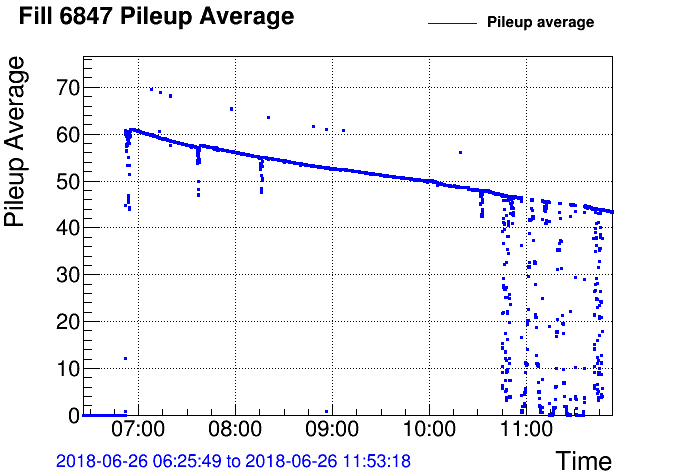
\includegraphics[width=0.55\linewidth]{plots/fill_6847_pileup_avg.png}
    \caption{
      Pile-up profile for LHC fill 6847. Two pile-up scans were performed between 11:00-11:30.
      \label{fig:fillpu6847}
    }
  \end{center}
\end{figure}

\begin{figure}[hbt]
  \begin{center}
    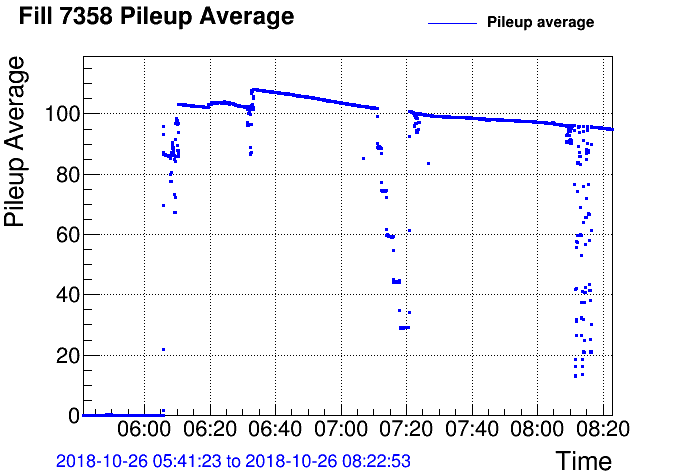
\includegraphics[width=0.55\linewidth]{plots/fill_7358_pileup_avg.png}
    \caption{
      Pile-up profile for LHC fill 7358. A pile-up scan was performed between  07:10-07:20.
      \label{fig:fillpu7358}
    }
  \end{center}
\end{figure}

\clearpage
\begin{figure}[hbt]
  \begin{center}

    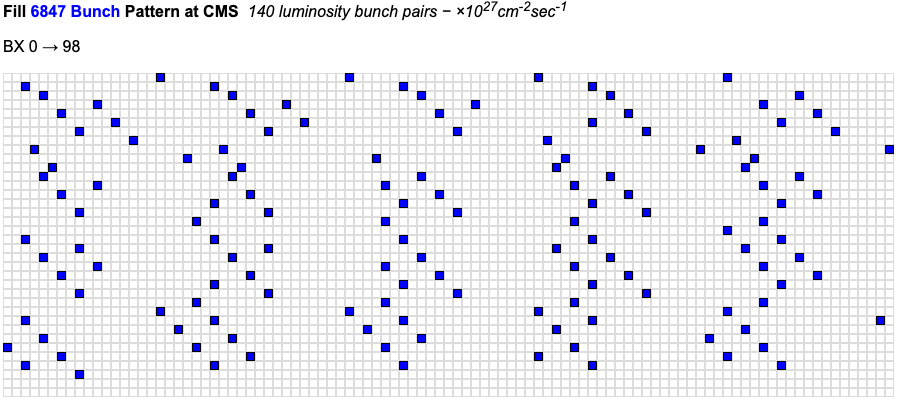
\includegraphics[width=0.99\linewidth]{plots/fillpattern_6847.png}
    \caption{
      Colliding bunch pattern for LHC fill 6847. 
    \label{fig:fill6847pattern}
    }

    \vspace{12pt}
    
    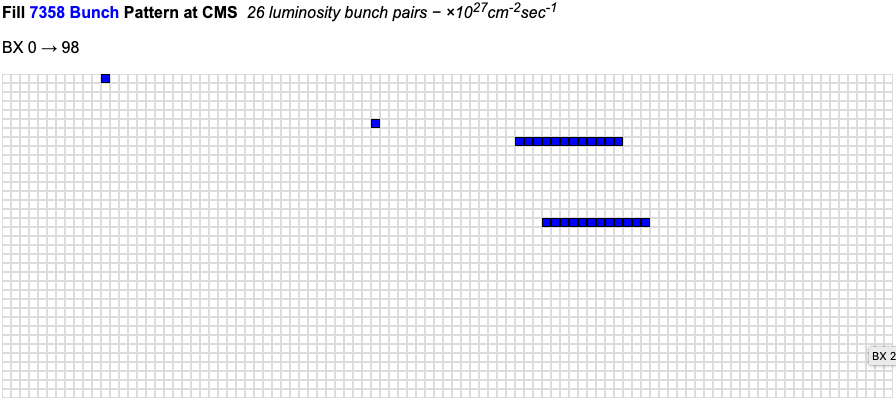
\includegraphics[width=0.99\linewidth]{plots/fillpattern_7358.png}
    \caption{
      Colliding bunch pattern for LHC fill 7358. 
    \label{fig:fill7358pattern}
    }

  \end{center}
\end{figure}


\clearpage
\newpage
\section{Pixel Cluster Counting (PCC) configuration}

\begin{figure}[t]
  \begin{center}
    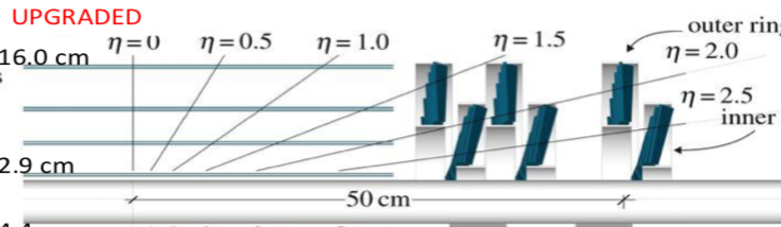
\includegraphics[width=0.9\linewidth]{plots/PixLayout.png}
    \caption{
      Layout of the Run II Pixel detector showing the 4 Barrel layers (0,1,2,3) and 3 Forward disks composed of 2 Panels each. 
    \label{fig:pixellayout}
    }
  \end{center}
\end{figure}


The layout of one quadrant of the Pixel detector used in CMS for  Run II is shown in Fig~\ref{fig:pixellayout}.
It is composed of a Barrel section with 4 layers and the Forward section with two Panels, each with 3 disks.
The Pixel sensors are read out by a total of 1856 modules.
A stability study comparing different periods in 2018 was used to exclude a list of modules which showed large variations between periods.
A total of 1387 modules are removed, this veto list can be found in Appendix~\ref{sec:appendix1} and maps per detector section are shown in figure~\ref{fig:pixelmodvetomap} and table~\ref{tab:pixveto}.
After the module veto the relative weights of each detector have the values shown in Figure~\ref{fig:pixelweights}.

\begin{table}[hc]
\caption{Number of vetoed modules per Pixel section.}
\label{tab:pixveto}
\begin{center}
\begin{tabular}{l|c|c}
\hline
\multirow{2}{*}{Section} & \multicolumn{2}{c}{$\#$ of Removed modules}  \\
  & $-$Side & $+$Side \\
\hline
BPIX layer 0 & - & - \\
BPIX layer 1 & 108 & 110 \\
BPIX layer 2 & 94  & 168 \\
BPIX layer 3 & 111 & 186 \\
FPIX Panel 0 & 122 & 122 \\
FPIX Panel 1 & 140 & 132 \\
\hline\hline
\end{tabular}
\end{center}
\end{table}


\newpage
\begin{figure}[hbt]
  \begin{center}

    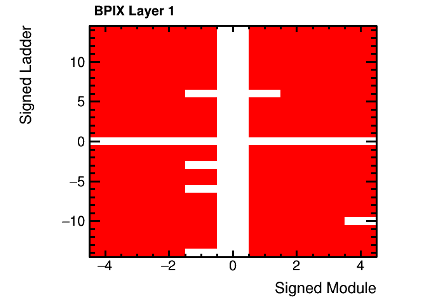
\includegraphics[width=0.45\linewidth]{plots/VetoMap_BPIX1.png}\\
    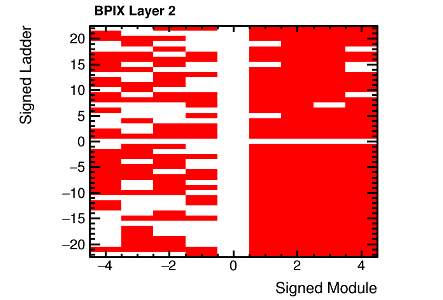
\includegraphics[width=0.45\linewidth]{plots/VetoMap_BPIX2.png}
    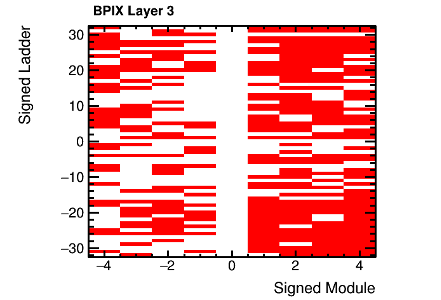
\includegraphics[width=0.45\linewidth]{plots/VetoMap_BPIX3.png}
    \vspace{20pt}
    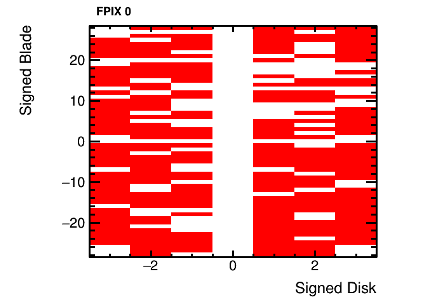
\includegraphics[width=0.45\linewidth]{plots/VetoMap_FPIX0.png}
    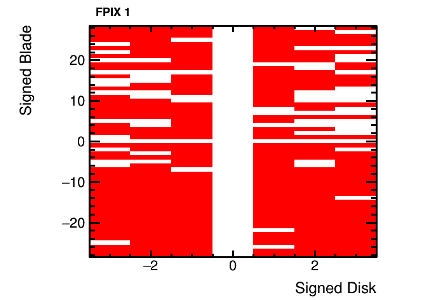
\includegraphics[width=0.45\linewidth]{plots/VetoMap_FPIX1.png}
    \caption{
      Maps of Pixel modules vetoed in the PCC luminosity computation. The veto list corresponds to the study performed using 2018 data including Run D period.
    \label{fig:pixelmodvetomap}
    }
  \end{center}
\end{figure}



\newpage
\begin{figure}[hc]
  \begin{center}
    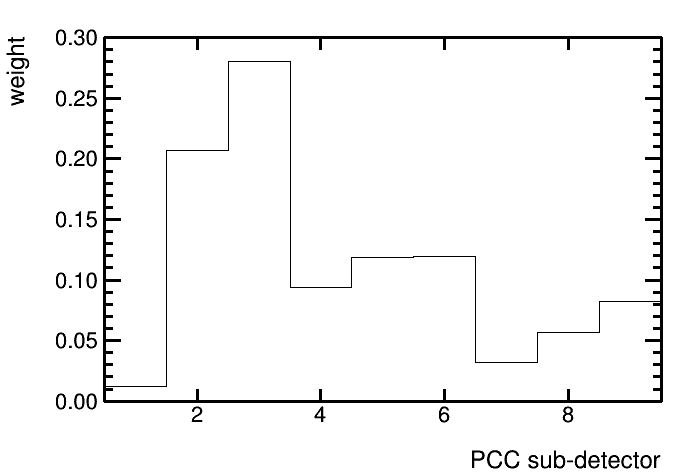
\includegraphics[width=0.7\linewidth]{plots/PCCWeights.png}
    \caption{
      Fraction of total clusters per each part of the Pixel detector. The weights are determined after applying the module veto list.
      Bins 1,2,3 correspond to the BPIX layers, bins 4,5,6 correspond to the FPIX Panel 0 disks (inner), and 7,8,9 to the FPIX Panel 1 disks (outer).
      \label{fig:pixelweights}
    }
  \end{center}
\end{figure}

\clearpage
\newpage
\section{Data sets and visible cross-sections}

For the PCC luminosity determination two types of data-sets are processed, Random trigger data for determination of ``afterglow'' corrections using the noise observed in non-colliding bunches, and ZeroBias data for the cluster counting in colliding bunches.
The data samples are stored in ALCARECO format in the CERN EOS system in the paths shown in Table~\ref{tab:datapaths}.

Additional data is needed to obtain the corresponding luminosity for the HF, PLT, and BCM luminometers.
For these detectors the BRIL data acquisition system (\emph{BRIL-DAQ}) is used and the data is stored in HD5 file format in special machines at Point 5 (\emph{brildev}).
The data samples used are shown in the Table~\ref{tab:datapathsbrildev}.
For these luminometers no additional corrections are applied, except for the HFOC residual afterglow.

The HF luminometer data in the hd5 files does not include final afterglow corrections for the HFOC algorithm.
These corrections have been obtained separately in ROOT histogram format from the Princeton group, and are currently stored in the following public directory:\\
\emph{/afs/cern.ch/user/j/jingyu/public/LUMI/for\_jose/}

The visible cross-sections used to normalize the data from each luminometer are listed in Table~\ref{tab:crossections}.
The values used for each luminometer differ from the ones listed in the 2018 PAS due to corrections which are needed for each detector as described in the table.




\clearpage
\begin{table}[h]
  \caption{Paths to the data used for the PCC luminosity determination (ZeroBias) and afterglow corrections (Random).
  The data paths are relative to the CERN eos system: $/eos/cms/store/$
  }
  \label{tab:datapaths}
  \footnotesize
  \begin{tabular}{l}
    \hline\hline
    Fill 6847:\\
data/Run2018B/AlCaLumiPixels/ALCARECO/AlCaPCCRandom-PromptReco-v2/000/318/675/\\ %00000/1E77B884-FF7A-E811-803C-FA163E76D066.root \\
data/Run2018B/AlCaLumiPixels0/ALCARECO/AlCaPCCZeroBias-PromptReco-v2/000/318/675/\\ %00000/9A8628CC-DF7A-E811-A671-FA163EDE4F34.root \\
data/Run2018B/AlCaLumiPixels1/ALCARECO/AlCaPCCZeroBias-PromptReco-v2/000/318/675/\\ %00000/16F2BA8F-D97A-E811-9385-FA163EA487EB.root \\
data/Run2018B/AlCaLumiPixels2/ALCARECO/AlCaPCCZeroBias-PromptReco-v2/000/318/675/\\ %00000/0677196F-D67A-E811-8E4E-FA163EF568AC.root \\
data/Run2018B/AlCaLumiPixels3/ALCARECO/AlCaPCCZeroBias-PromptReco-v2/000/318/675/\\ %00000/D8813469-D57A-E811-84C8-FA163E18DCD1.root \\
data/Run2018B/AlCaLumiPixels4/ALCARECO/AlCaPCCZeroBias-PromptReco-v2/000/318/675/\\ %00000/DECE9555-FD7A-E811-A11F-FA163E5B62DF.root \\
data/Run2018B/AlCaLumiPixels5/ALCARECO/AlCaPCCZeroBias-PromptReco-v2/000/318/675/\\ %00000/BA53B331-EE7A-E811-8AC2-02163E019EC5.root \\
data/Run2018B/AlCaLumiPixels6/ALCARECO/AlCaPCCZeroBias-PromptReco-v2/000/318/675/\\ %00000/4E162320-E47A-E811-B5EA-FA163EB7AC61.root \\
data/Run2018B/AlCaLumiPixels7/ALCARECO/AlCaPCCZeroBias-PromptReco-v2/000/318/675/\\ %00000/22A4C262-E17A-E811-AFEF-FA163E336245.root \\
data/Run2018B/AlCaLumiPixels8/ALCARECO/AlCaPCCZeroBias-PromptReco-v2/000/318/675/\\ %00000/F69D7D47-E77A-E811-9C74-FA163E163082.root \\
data/Run2018B/AlCaLumiPixels9/ALCARECO/AlCaPCCZeroBias-PromptReco-v2/000/318/675/\\ %00000/680CF7EB-D47A-E811-BAFB-FA163EA487EB.root \\
\hline
    Fill 7358:\\
express/Run2018E/StreamALCALUMIPIXELSEXPRESS/ALCARECO/AlCaPCCRandom-Express-v1/000/325/309/\\ %00000/4C63A580-3BA2-0D4E-A447-E5A980883D1E.root \\
data/Run2018E/AlCaLumiPixels1/ALCARECO/AlCaPCCZeroBias-PromptReco-v1/000/325/309/\\ %00000/3993D954-4C5C-2247-8935-A8D6019151B7.root \\
data/Run2018E/AlCaLumiPixels2/ALCARECO/AlCaPCCZeroBias-PromptReco-v1/000/325/309/\\ %00000/E56486D8-15C1-6E47-BB5B-C798DC7B35E5.root \\
data/Run2018E/AlCaLumiPixels3/ALCARECO/AlCaPCCZeroBias-PromptReco-v1/000/325/309/\\ %00000/7136F0DC-3A4B-4445-8AB4-9EA9D9BE16F6.root \\
data/Run2018E/AlCaLumiPixels4/ALCARECO/AlCaPCCZeroBias-PromptReco-v1/000/325/309/\\ %00000/B0920DA1-D6B5-1545-BA56-7597EB33FD47.root \\
data/Run2018E/AlCaLumiPixels5/ALCARECO/AlCaPCCZeroBias-PromptReco-v1/000/325/309/\\ %00000/96C74CCD-682A-5D47-9AC8-BE229BD27DA3.root \\
data/Run2018E/AlCaLumiPixels6/ALCARECO/AlCaPCCZeroBias-PromptReco-v1/000/325/309/\\ %00000/415CC662-DB7D-F74F-9FB9-AB878EF770C5.root \\
data/Run2018E/AlCaLumiPixels7/ALCARECO/AlCaPCCZeroBias-PromptReco-v1/000/325/309/\\ %00000/A4711D16-DB69-7447-93FF-4CA53B476927.root \\
data/Run2018E/AlCaLumiPixels8/ALCARECO/AlCaPCCZeroBias-PromptReco-v1/000/325/309/\\ %00000/CC2437DB-E2CD-444D-832A-BAF3C7592C21.root \\
data/Run2018E/AlCaLumiPixels9/ALCARECO/AlCaPCCZeroBias-PromptReco-v1/000/325/309/\\ %00000/E7DA9BE1-28F3-3A40-98A9-A22761530735.root \\
\hline\hline
  \end{tabular}
\end{table}

\vspace{24pt}
\begin{table}[h]
\begin{center}
\caption{Paths to the data used for the HF, BCM, and PLT luminometers. This data is stored in the \emph{brildev} system at Point 5.}
  \label{tab:datapathsbrildev}
 % \footnotesize
  \begin{tabular}{c|l}
    \hline\hline
Fill & Data Path \\
6847 &  /brildata/vdmdata18/6847\_1806261047\_1806261133.hd5 \\
7358 & /brildata/vdmdata18/7358\_1810260704\_1810260726.hd5  \\
    \hline\hline
  \end{tabular}
\end{center}
\end{table}


\vspace{24pt}
\begin{table}[h]
  \caption{Visible cross-sections used for each luminometer in this analysis. The differences with respect to the values in the 2018 PAS \cite{CMS-PAS-LUM-18-002} are described in the third column.}
  \label{tab:crossections}
    \begin{tabular}{l|c|c}
      \hline
      Luminometer & $\sigma_{vis}$ & Difference w.r.t \cite{CMS-PAS-LUM-18-002}\\
      \hline
      PCC   &  3140  $mb$     & This value corresponds to a tighter module veto list. \\
      HFOC  &  797.5 $\mu b$  & This value is further corrected by 0.987 for radiation damage in Fill 7358. \\
      BCM1F &  203.2 $\mu b$  &  ?? \\
      PLT   &  305   $\mu b$  & Corrected using emmittance scan data. \\
      \hline\hline
    \end{tabular}
\end{table}

\clearpage
\newpage
\section{Afterglow corrections}

The PCC and HF luminometers  require corrections for the so called ``afterglow'' effects, noise induced in bunch crossings following colliding bunch crossings.
Two corrections have been previously developed: Type-1 refers to a spill over into the bunch crossing immediately following an active bunch crossing due to charge residuals in the pixel sensors, the second Type-2 refers to exponentially decaying noise created by activated material.
The models for both corrections are normalized using data from empty bunch crossings recorded with RANDOM triggers.
The corrections are stored in the Conditions Database (CONDDB) during the Prompt Calibration Loop (PCL).
The PCC values obtained from the ZEROBIAS trigger data are then corrected in an offline analysis.

The afterglow corrections are normally calculated for an integrated range of lumi sections to improve the statistical precision, for PCC every 50 LS while for HFOC every 20. In this study the PCC corrections were determined privately every 10 LS to capture variations during $\mu$-scans.
Example corrections (Type-1 and Type-2 combined) are showin in Figure~\ref{fig:afterglow}.
For fill 6847 the corrections have values of 1.0 due to the single bunch pattern.

\begin{figure}[t]
  \begin{center}
    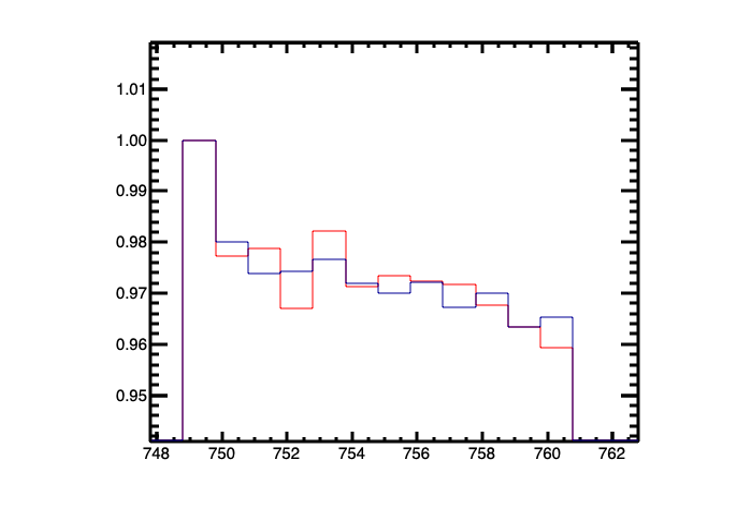
\includegraphics[width=0.47\linewidth]{plots/AfterglowCorrections_7358_PCC.png}
    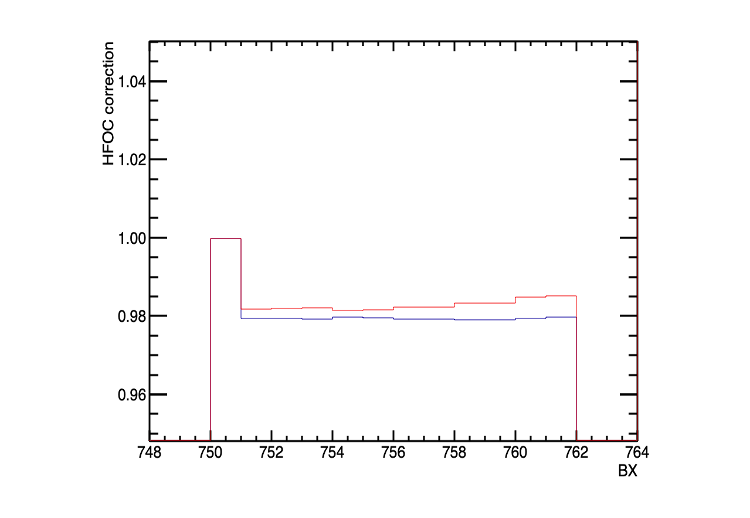
\includegraphics[width=0.47\linewidth]{plots/AfterglowCorrections_7358_HFOC.png}
    \caption{
      Afterglow corrections as a function of bcid for one bunch train in fill 7358.
      For PCC (HFOC) the blue histogram corresponds to lumi sections 1-11 (1-20), while the red histogram to lumi sections 23-33 (21-40).
    \label{fig:afterglow}
    }
  \end{center}
\end{figure}


\clearpage
\newpage
\section{Time selections}

The luminometer data corresponding to the $\mu$-scans is selected by applying selections on the time stamps.
The selections remove luminosity values when the LHC beam conditions are in transition.
The time selections are best determined from one of the luminometers read by the BRIL-DAQ as the temporal granularity has ``nibble'' resolution ($\sim$2s), while the PCC luminosity values are determined every lumi section ($\sim$23s).

Figure~\ref{fig:lumivstime} shows the luminosity vs. time for the HFOC luminometer and the transition time stamps that were determined from these data.
The absolute time stamp values in seconds are the following:
\begin{itemize}
\item Fill 6847 : 1530010610, 1530010615, 1530010670, 1530010721, 1530010772, 1530010824, 1530010875, 1530010926, 1530010978, 1530011031, 1530011082, 1530011133, 1530011184, 1530011235, 1530011287, 1530011339, 1530011393, 1530011441, 1530011489, 1530011537, 1530011585, 1530011633, 1530011681, 1530011729, 1530011761, 1530011811, 1530011863, 1530011914, 1530011966, 1530012019, 1530012070, 1530012122, 1530012173, 1530012225, 1530012277, 1530012328, 1530011400
\item Fill 7358 : 1540537829, 1540537864, 1540537940, 1540538037, 1540538158, 1540538277, 1540538446, 1540538429
\end{itemize}

All data  within 24 seconds of these transitions times are excluded from the analysis, in the case of PCC the luminosity sections with time stamps in these windows are removed.
The data for luminometers with nibble granualurity (HFOC, PLT, BCM) are then averaged within the corresponding  lumisections for comparison with PCC. 
The PCC and HFOC luminosity values per lumisection before and after the time selections are shown in Figure~\ref{fig:lumivsls}.


\begin{figure}[t]
  \begin{center}
    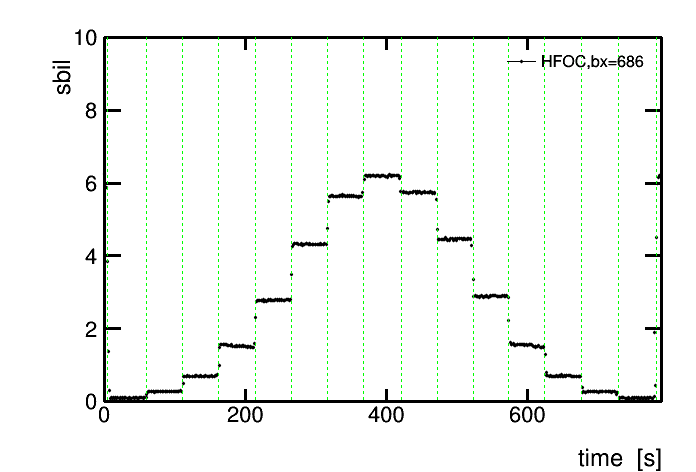
\includegraphics[width=0.47\linewidth]{plots/plot_lumi_vstime_6847.png}
    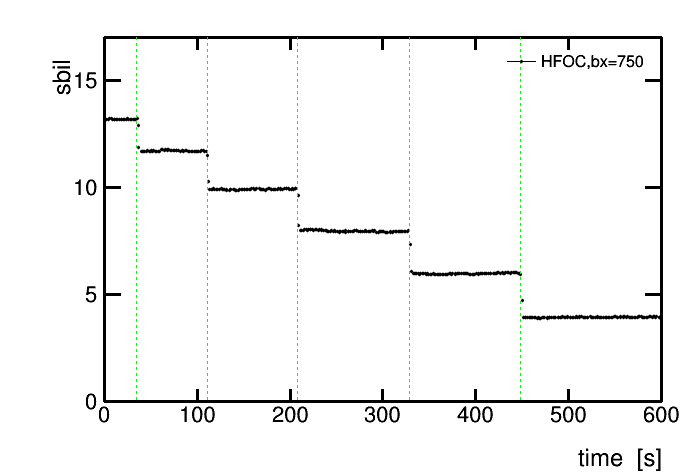
\includegraphics[width=0.47\linewidth]{plots/plot_lumi_vstime_7358.png}
    \caption{
      SBIL data for the HFOC covering the time range of one $\mu$-scan in Fill 6847 (left) and Fill 7358 (right). The vertical lines mark the time stamps determined from this data where the LHC beam parameters are changed.
    \label{fig:lumivstime}
    }
  \end{center}
\end{figure}


\newpage

\begin{figure}[t]
  \begin{center}
    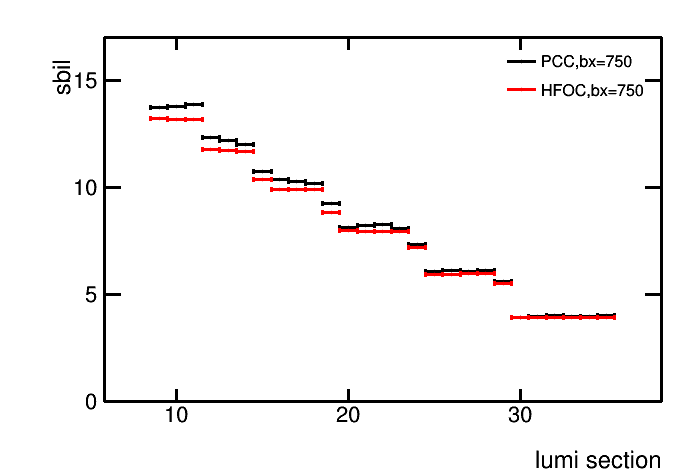
\includegraphics[width=0.6\linewidth]{plots/plot_lumi_vsls_7358_before.png}
    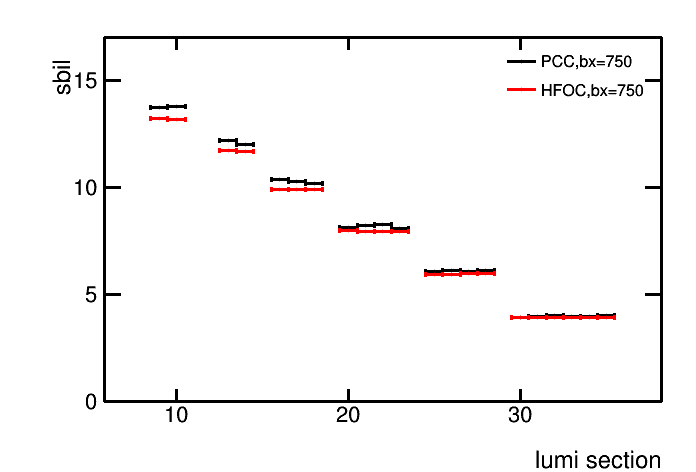
\includegraphics[width=0.6\linewidth]{plots/plot_lumi_vsls_7358_after.png}
    \caption{
    PCC and HFOC single bunch instantenous luminosity (SBIL) for one bunch crossing in Fill 7358 before (top) and after (bottom) applying the time selections.
    \label{fig:lumivsls}
    }
  \end{center}
\end{figure}

\clearpage
\newpage
\section{Relative linearity determination}

The determination of the relative linearity between two luminometers requires fitting for the slope in the ratio of the SBIL values as a function of SBIL.
In the nominal comparison the HFOC is chosen as a reference luminometer due to its good statistical precision and stability.
The linearity is studied for individual bunch crossings after the corrections and selections described before.

In order to assign an uncertainty on the PCC/HFOC ratio at a given SBIL, ratio values computed for individual lumisections are grouped and averaged if their reference SBIL values are within 0.5.
The uncertainty is assigned as the standard deviation of the ratios used in the average.
Figure~\ref{fig:sbilratiomethod} illustrates the method, the resulting graph is fit using a linear function.


In Figures~\ref{fig:sbilratios6847} and \ref{fig:sbilratios7358} the linearity fits are shown for the single and leading bunches in fill 6847 and 7358.
Figures~\ref{fig:sbilratiosresults6847} and \ref{fig:sbilratiosresults7358} summarize  the fit parameter results.


Figure~\ref{fig:sbilratios_dets} compares the correlations and ratios between different luminometers for fill 7358.

\begin{figure}[t]
  \begin{center}
    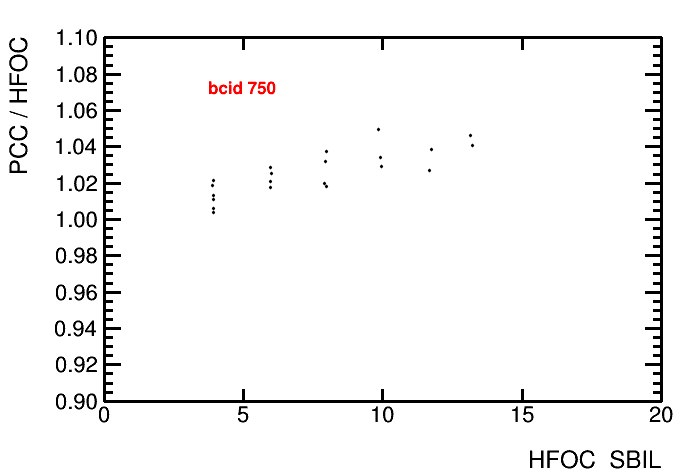
\includegraphics[width=0.47\linewidth]{plots/plot_det_linearity_perbx_pcc_7358_750_scatter.png}
    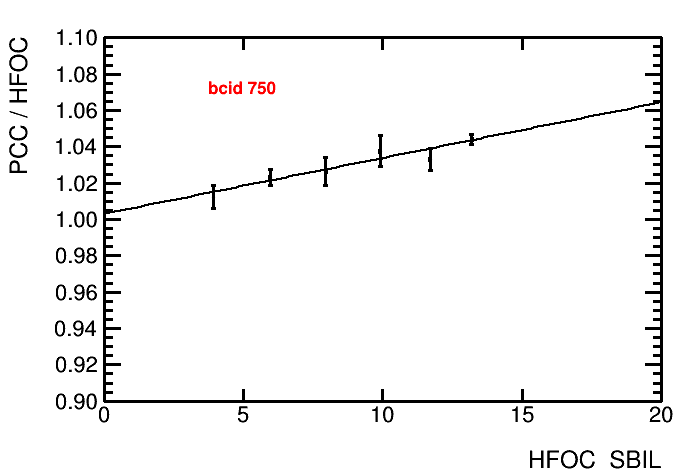
\includegraphics[width=0.47\linewidth]{plots/plot_det_linearity_perbx_pcc_7358_750_avg.png}
    \caption{
      PCC / HFOC  SBIL ratios as a function of HFOC SBIL for one bunch crossing in Fill 7358.
      The graphs illustrate the method for determining the average ratio at a given SBIL value as described in the text.
    \label{fig:sbilratiomethod}
    }
  \end{center}
\end{figure}

\clearpage
\begin{figure}[t]
  \begin{center}
    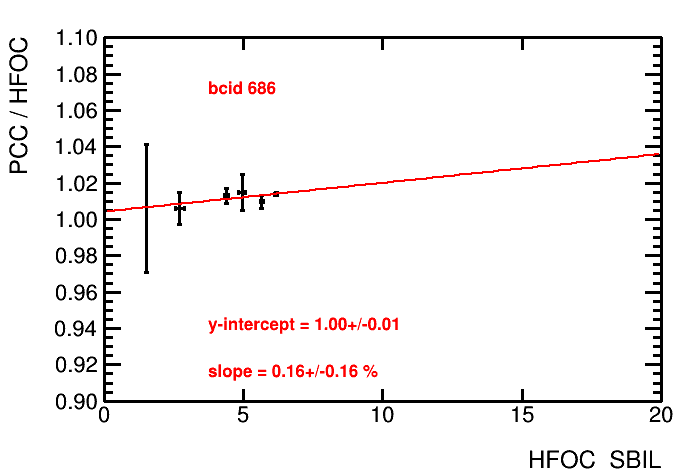
\includegraphics[width=0.47\linewidth]{plots/sbilratios_singles/plot_det_linearity_perbx_pcc_6847_686.png}
    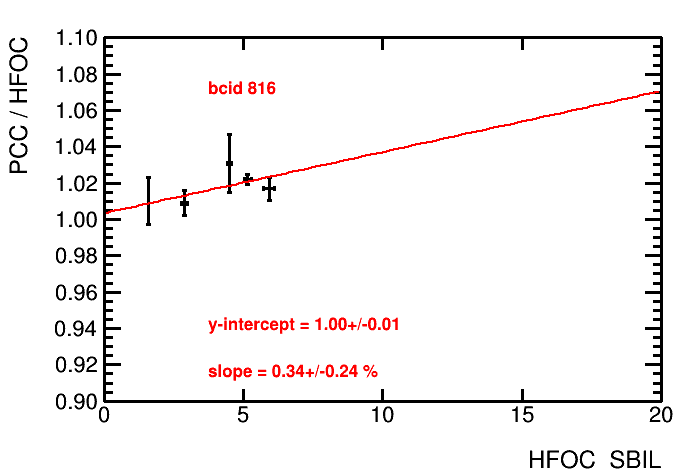
\includegraphics[width=0.47\linewidth]{plots/sbilratios_singles/plot_det_linearity_perbx_pcc_6847_816.png}
    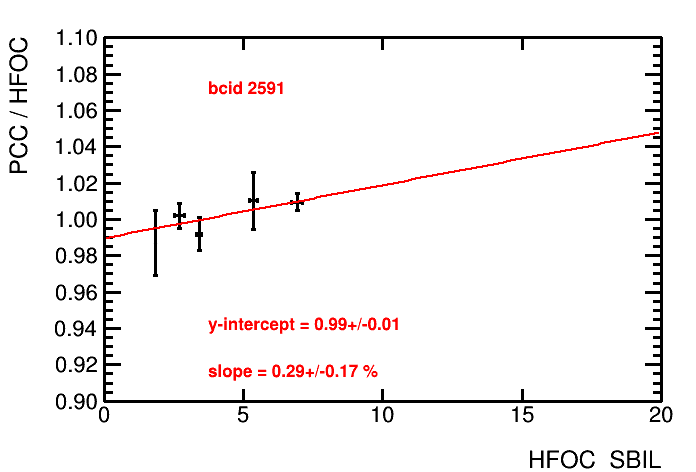
\includegraphics[width=0.47\linewidth]{plots/sbilratios_singles/plot_det_linearity_perbx_pcc_6847_2591.png}
    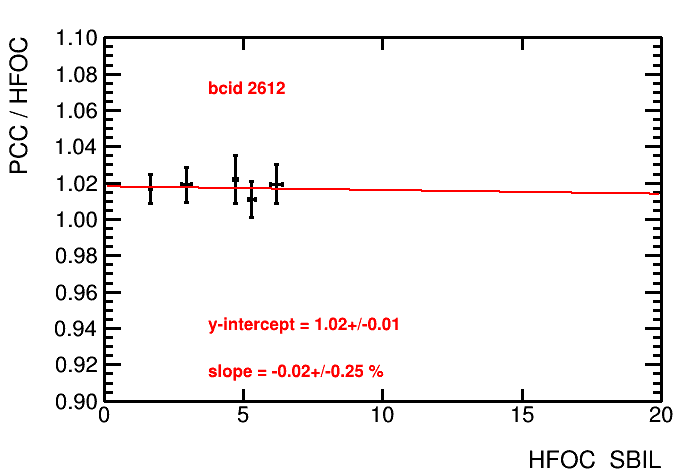
\includegraphics[width=0.47\linewidth]{plots/sbilratios_singles/plot_det_linearity_perbx_pcc_6847_2612.png}
    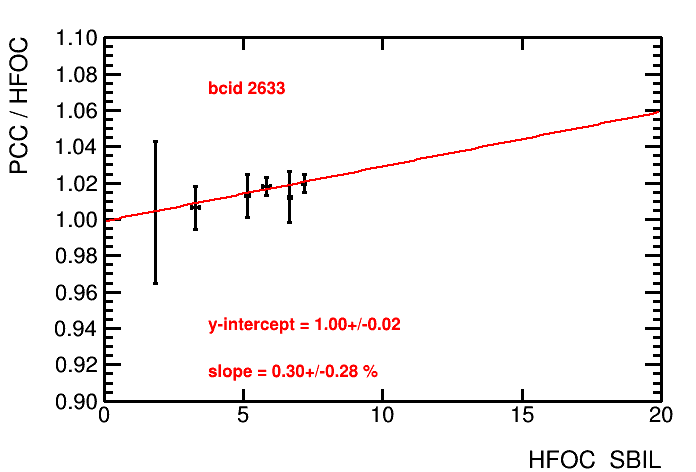
\includegraphics[width=0.47\linewidth]{plots/sbilratios_singles/plot_det_linearity_perbx_pcc_6847_2633.png}
    \caption{
      Ratio of PCC over HFOC single bunch instantenous luminosity (SBIL) as a function of SBIL for the 5 high statistics bunches in Fill 6847.
      The points and error bars are determined as described in the text.
    \label{fig:sbilratios6847}
    }
  \end{center}
\end{figure}

\clearpage
\begin{figure}[t]
  \begin{center}
    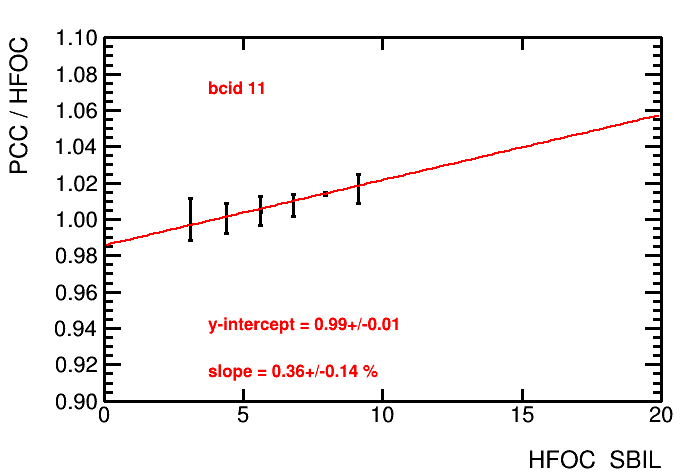
\includegraphics[width=0.47\linewidth]{plots/sbilratios_singles/plot_det_linearity_perbx_pcc_7358_11.png}
    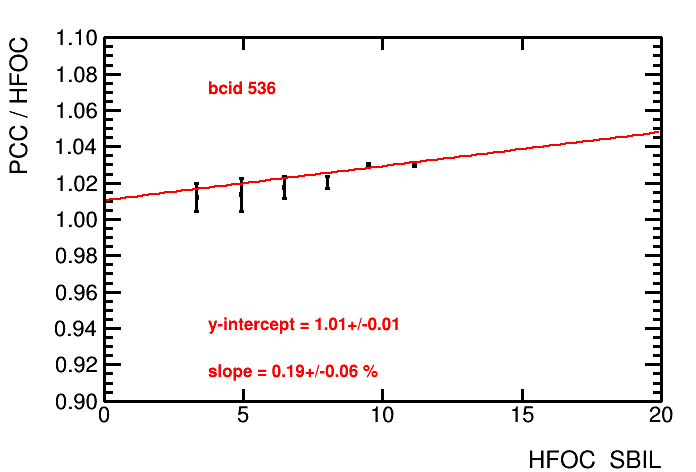
\includegraphics[width=0.47\linewidth]{plots/sbilratios_singles/plot_det_linearity_perbx_pcc_7358_536.png}
    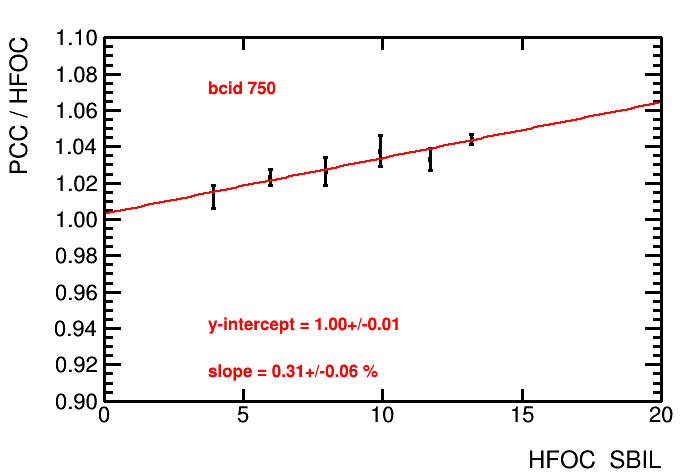
\includegraphics[width=0.47\linewidth]{plots/sbilratios_singles/plot_det_linearity_perbx_pcc_7358_750.png}
    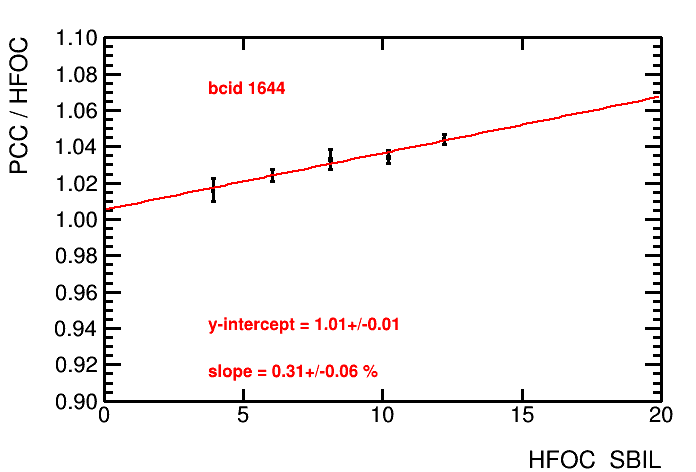
\includegraphics[width=0.47\linewidth]{plots/sbilratios_singles/plot_det_linearity_perbx_pcc_7358_1644.png}
    \caption{
      Ratio of PCC over HFOC single bunch instantenous luminosity (SBIL) as a function of SBIL for the 2 solo and 2 leading  bunches in Fill 7358.
      The points and error bars are determined as described in the text.
      \label{fig:sbilratios7358}
    }
  \end{center}
\end{figure}

\clearpage
\begin{figure}[t]
  \begin{center}
    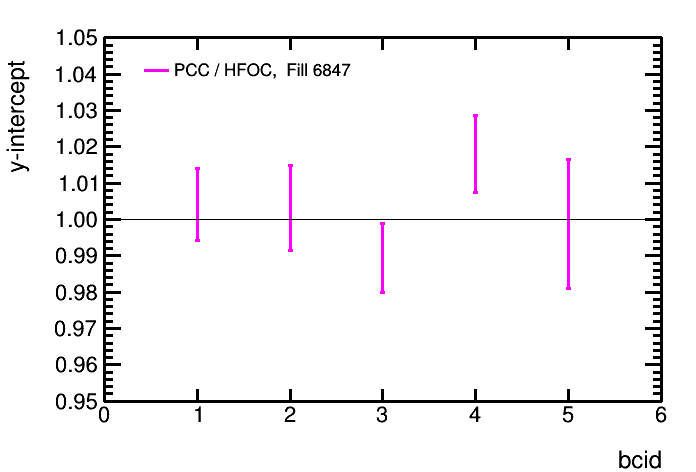
\includegraphics[width=0.47\linewidth]{plots/sbilratios_singles/plot_det_linearity_perbx_y0_6847.png}
    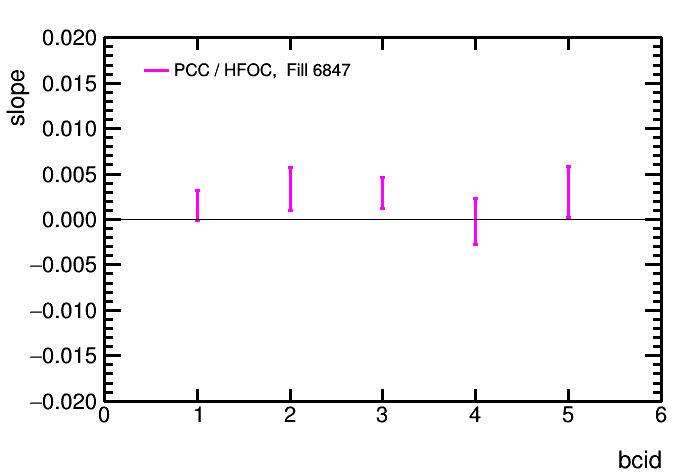
\includegraphics[width=0.47\linewidth]{plots/sbilratios_singles/plot_det_linearity_perbx_slope_6847.png}
    \caption{
      y-intercept (left) and slope (right) for the linear fits to the ratios of PCC/HFOC v.s. SBIL for the 5 high statistics bunches in Fill 6847.
      \label{fig:sbilratiosresults6847}
    }
  \end{center}
\end{figure}

\begin{figure}[t]
  \begin{center}
    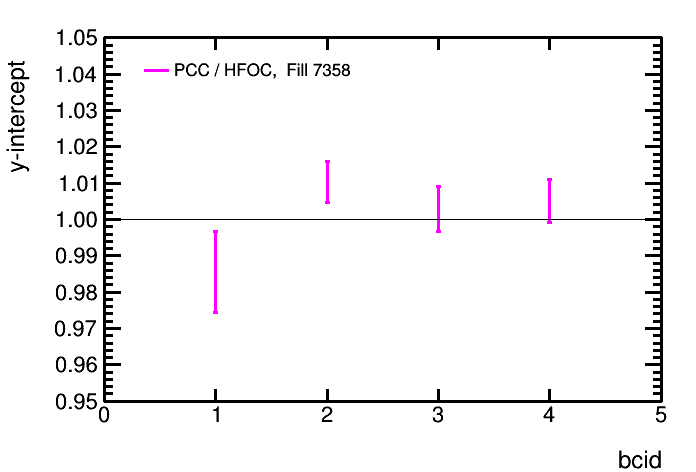
\includegraphics[width=0.47\linewidth]{plots/sbilratios_singles/plot_det_linearity_perbx_y0_7358.png}
    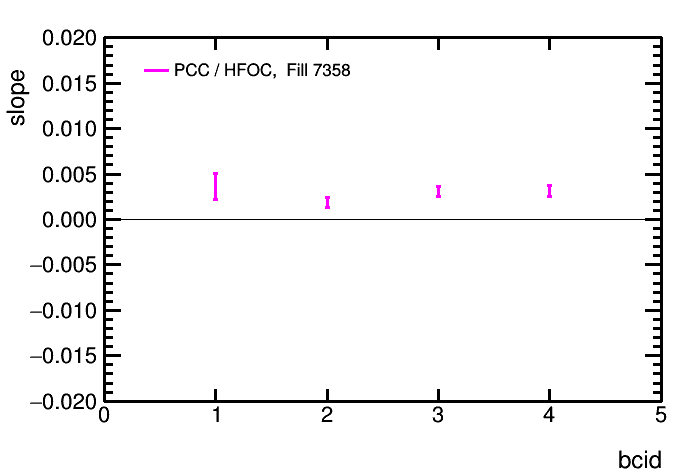
\includegraphics[width=0.47\linewidth]{plots/sbilratios_singles/plot_det_linearity_perbx_slope_7358.png}
    \caption{
      y-intercept (left) and slope (right) for the linear fits to the ratios of PCC/HFOC v.s. SBIL for the 2 solo and 2 leading  bunches in Fill 7358.
      \label{fig:sbilratiosresults7358}
    }
  \end{center}
\end{figure}


\clearpage
\begin{figure}[t]
  \begin{center}
    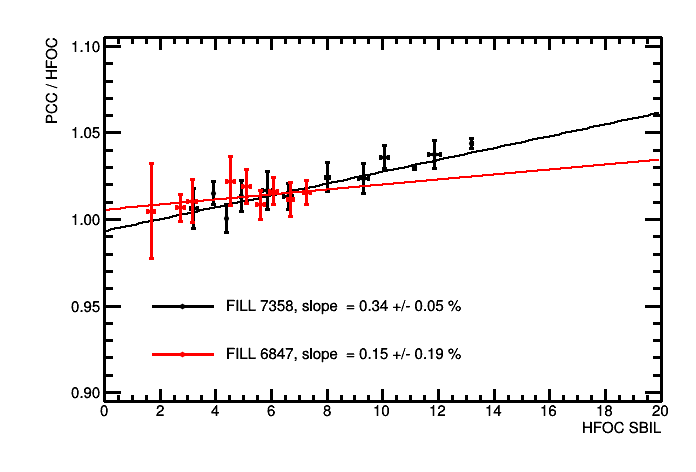
\includegraphics[width=0.7\linewidth]{plots/sbilratios_singles_combined/compareFills_graph_fillstogether.png}
    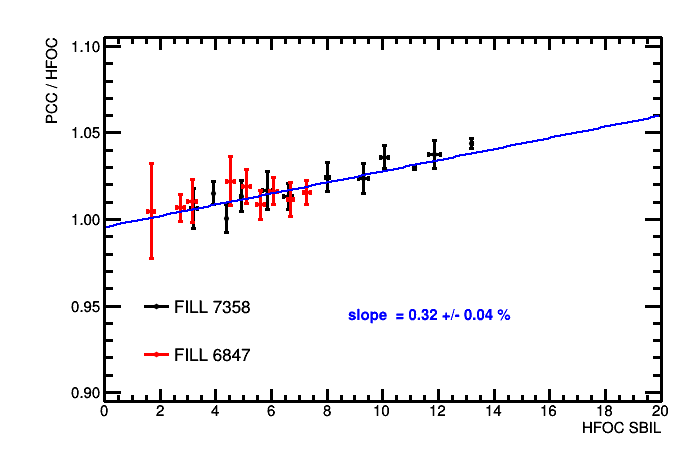
\includegraphics[width=0.7\linewidth]{plots/sbilratios_singles_combined/compareFills_graph_fillstogether_onefit.png}
    \caption{
      Comparison of the ratio of PCC / HFOC after combining all leading and solo bunches in fills 6847 and 7358.
      The data points and uncertainties are determined as described in the text.
      The fills are fit separately (top) and together (bottom).
      \label{fig:sbilratiosresultscombined}
    }
  \end{center}
\end{figure}


\clearpage
\begin{figure}[t]
  \begin{center}
    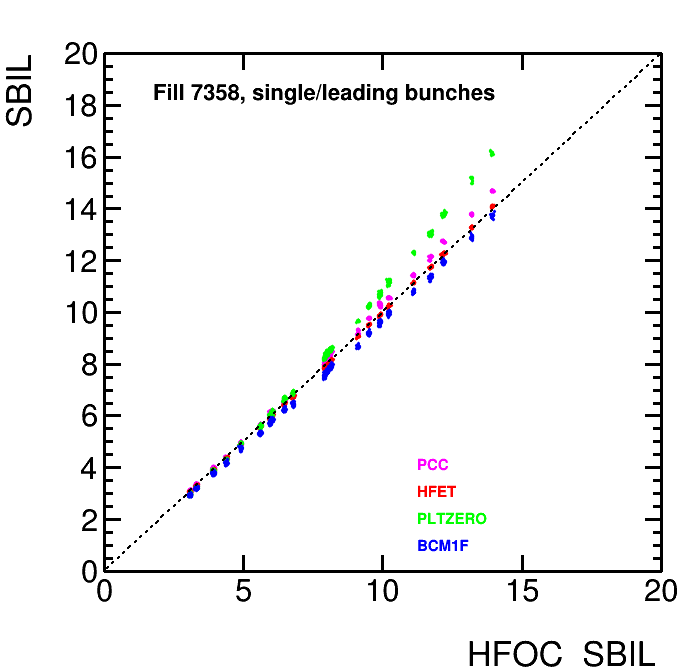
\includegraphics[width=0.47\linewidth]{plots/sbilratios_singles/plot_linearity_det_correlation.png}
    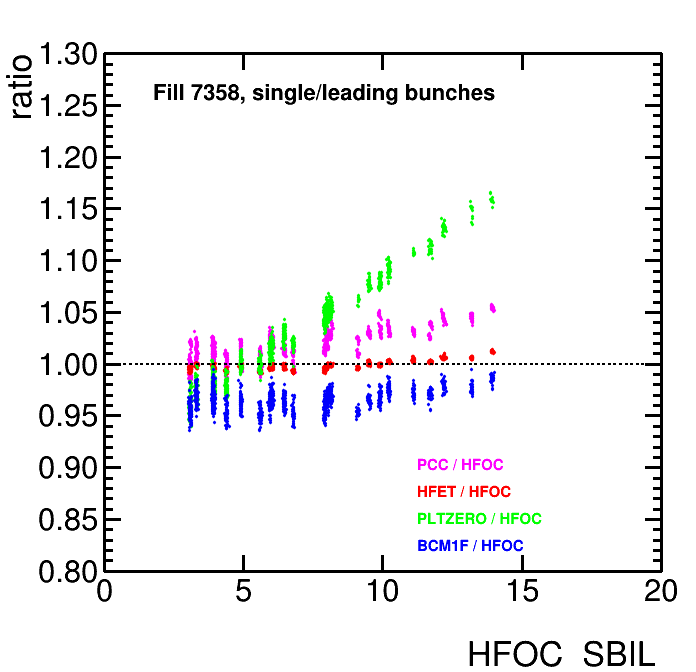
\includegraphics[width=0.47\linewidth]{plots/sbilratios_singles/plot_linearity_det_correlation_ratio.png}
    \caption{
      Correlations (left) and ratios (right) of the SBIL values between different luminometers in Fill 7358.
    \label{fig:sbilratios_dets}
    }
  \end{center}
\end{figure}

\clearpage
\newpage
\section{Train effects}
The dependence of the linearity fit results as a function of  the bunch crossing in the trains is shown in Figures~\ref{fig:fill7358trainresults}.
A systematic drop in the slope is observed as the colliding bunch is farther from the leading bunch.
In order to check if this trend may be caused by the afterglow corrections a check was performed as shown in Appendix~\ref{sec:appendix2} where the PCC and HFOC afterglow corrections are removed, however the change in the slope values is small.

Comparisons to other luminometers show a similar systematic trend for HFET and BCM1F (Figures~\ref{fig:fill7358trainslope_hfet} and \ref{fig:fill7358trainslope_bcm}).
In the case of PLT (Figure~\ref{fig:fill7358trainslope_plt}) the trend is less visible except for the leading bunch where a strong negative slope is obtained.

The effect was further studied by reprocessing the PCC data while modifying the module veto list to select different parts of the Pixel detector, these results are shown in Figure~\ref{fig:fill7358trainslope_pccparts}.
In these graphs it is observed that BPIX layer 1, FPIX Panel 1 all disks, and FPIX Panel 2 disks 1 show the trend, while the remaining parts are more stable.

\begin{figure}[t]
  \begin{center}
    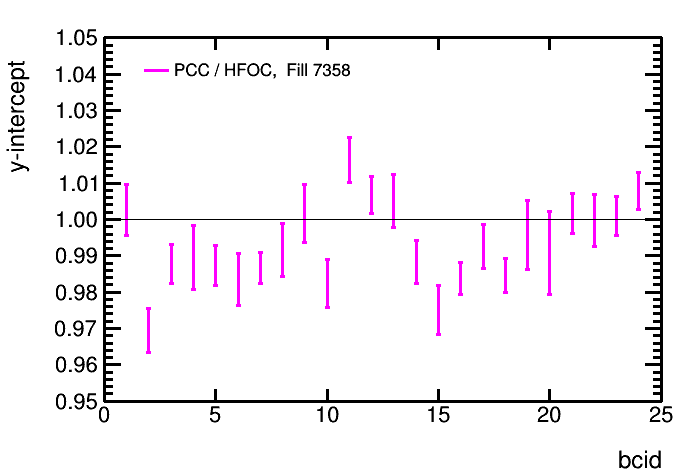
\includegraphics[width=0.47\linewidth]{plots/sbilratios_trains_Fill7358/plot_det_linearity_perbx_y0_7358.png}
    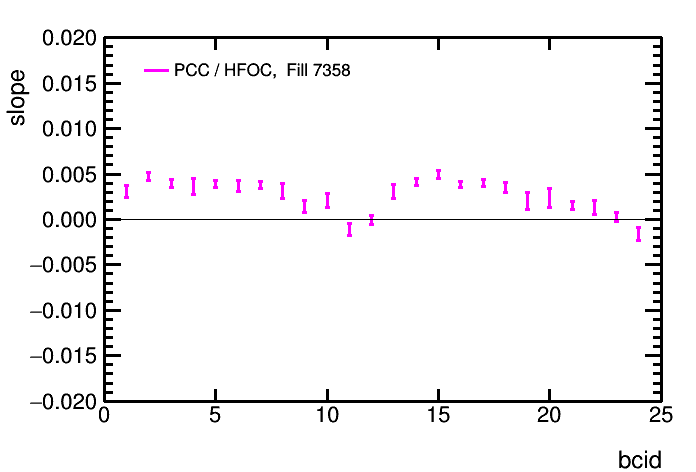
\includegraphics[width=0.47\linewidth]{plots/sbilratios_trains_Fill7358/plot_det_linearity_perbx_slope_7358.png}
    \caption{
      y-intercept and slope values obtained from the linearity fits for the 24 bunches in the two trains of Fill 7358.
      \label{fig:fill7358trainresults}
    }
  \end{center}
\end{figure}



\clearpage
\begin{figure}[t]
  \begin{center}
    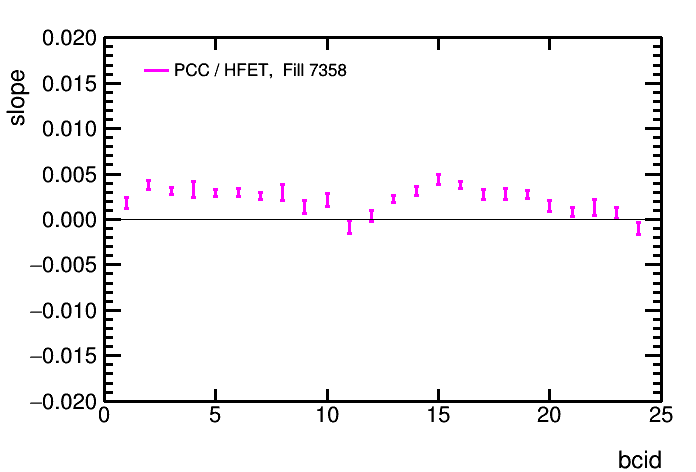
\includegraphics[width=0.47\linewidth]{plots/sbilratios_trains_Fill7358/plot_det_linearity_perbx_slope_7358_hfet.png}
    \caption{
      Slope values obtained from the linearity fits for the 24 bunches in the two trains of Fill 7358, in this plot the PCC is compared to the HFET luminometer.
      \label{fig:fill7358trainslope_hfet}
    }
  \end{center}
\end{figure}

\begin{figure}[t]
  \begin{center}
    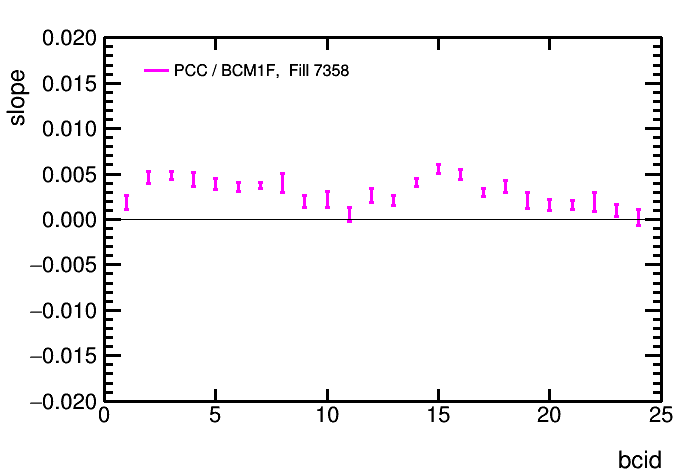
\includegraphics[width=0.47\linewidth]{plots/sbilratios_trains_Fill7358/plot_det_linearity_perbx_slope_7358_bcm.png}
    \caption{
      Slope values obtained from the linearity fits for the 24 bunches in the two trains of Fill 7358, in this plot the PCC is compared to the BCM1F luminometer.
      \label{fig:fill7358trainslope_bcm}
    }
  \end{center}
\end{figure}

\begin{figure}[t]
  \begin{center}
    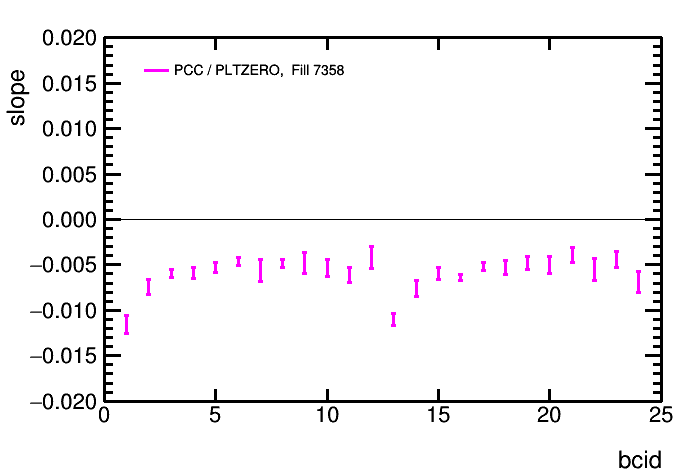
\includegraphics[width=0.47\linewidth]{plots/sbilratios_trains_Fill7358/plot_det_linearity_perbx_slope_7358_plt.png}
    \caption{
      Slope values obtained from the linearity fits for the 24 bunches in the two trains of Fill 7358, in this plot the PCC is compared to the PLTZERO luminometer.
      \label{fig:fill7358trainslope_plt}
    }
  \end{center}
\end{figure}


\clearpage
\begin{figure}[t]
  \begin{center}
    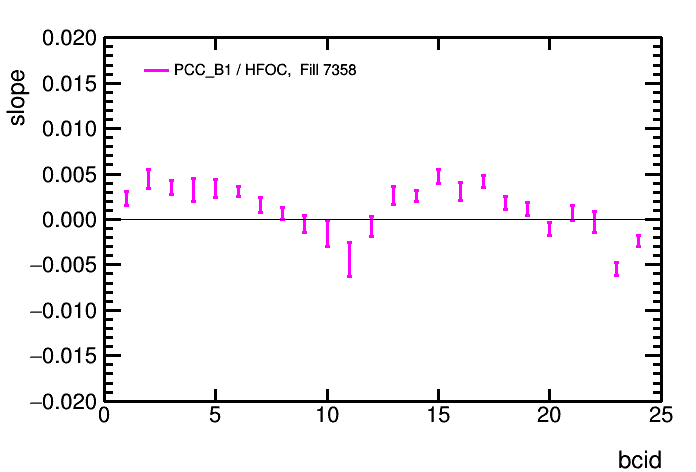
\includegraphics[width=0.32\linewidth]{plots/sbilratios_trains_Fill7358/plot_det_linearity_perbx_slope_7358_B1.png}
    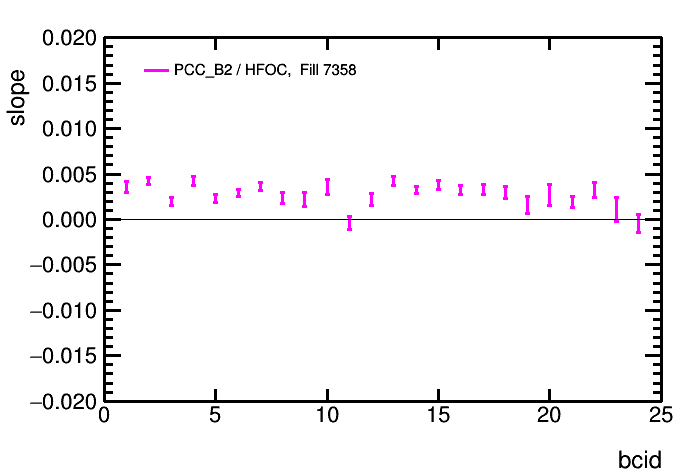
\includegraphics[width=0.32\linewidth]{plots/sbilratios_trains_Fill7358/plot_det_linearity_perbx_slope_7358_B2.png}
    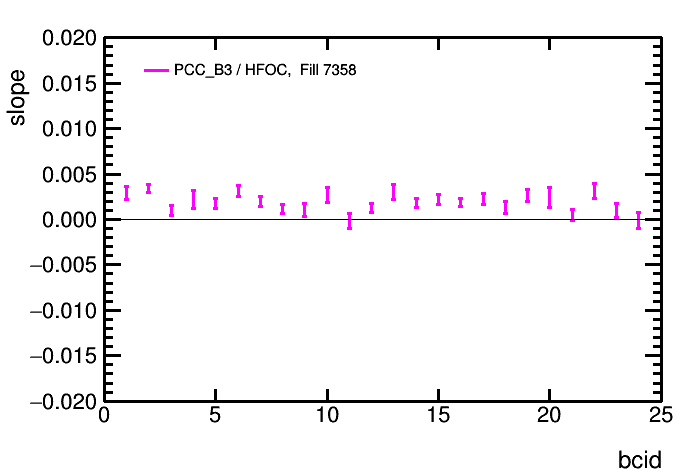
\includegraphics[width=0.32\linewidth]{plots/sbilratios_trains_Fill7358/plot_det_linearity_perbx_slope_7358_B3.png}
    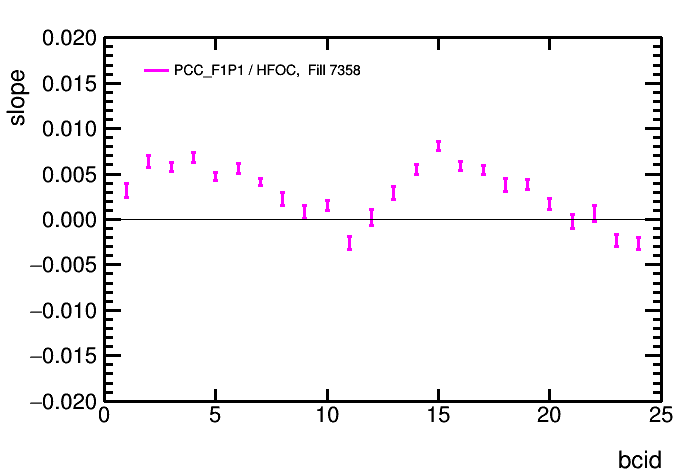
\includegraphics[width=0.32\linewidth]{plots/sbilratios_trains_Fill7358/plot_det_linearity_perbx_slope_7358_F1p1.png}
    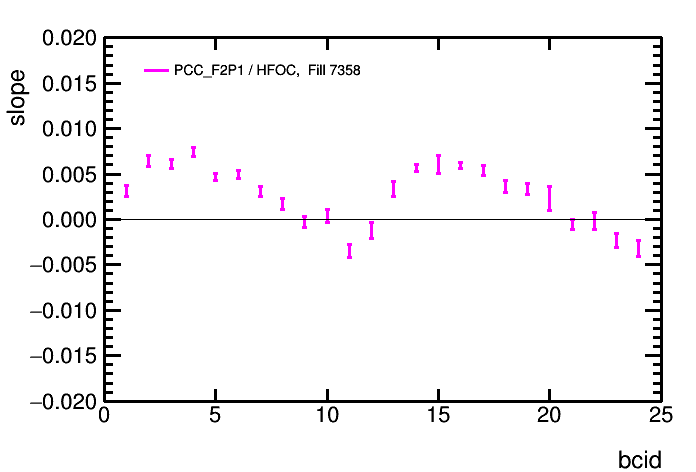
\includegraphics[width=0.32\linewidth]{plots/sbilratios_trains_Fill7358/plot_det_linearity_perbx_slope_7358_F2p1.png}
    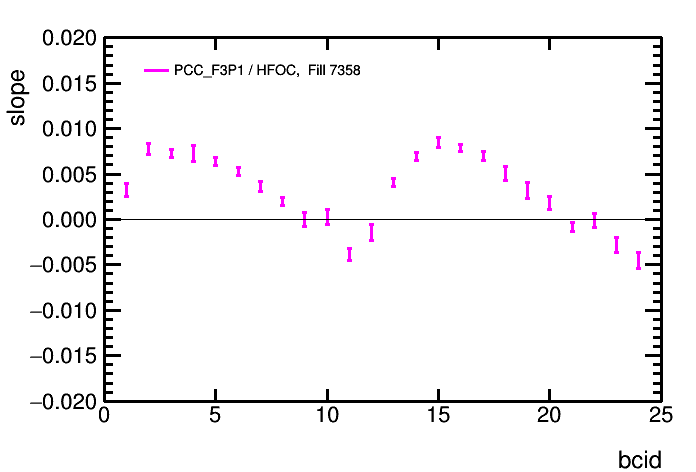
\includegraphics[width=0.32\linewidth]{plots/sbilratios_trains_Fill7358/plot_det_linearity_perbx_slope_7358_F3p1.png}
    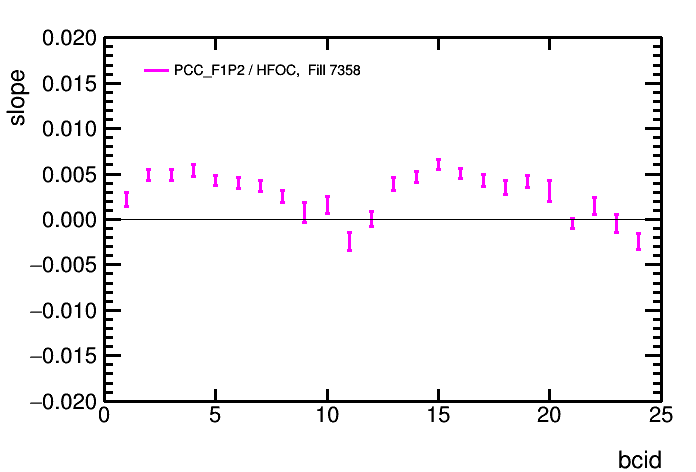
\includegraphics[width=0.32\linewidth]{plots/sbilratios_trains_Fill7358/plot_det_linearity_perbx_slope_7358_F1p2.png}
    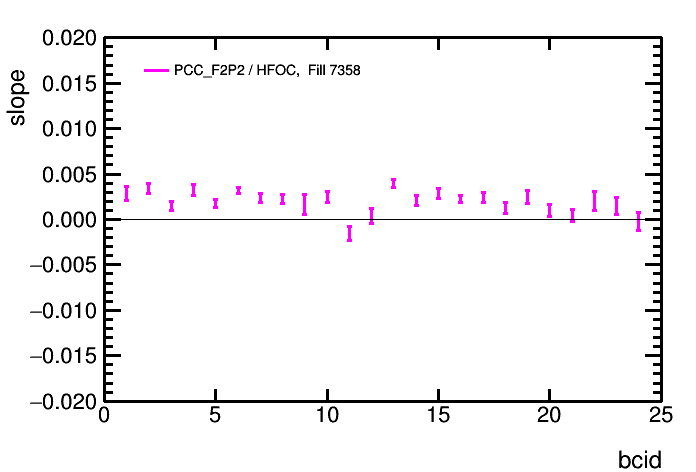
\includegraphics[width=0.32\linewidth]{plots/sbilratios_trains_Fill7358/plot_det_linearity_perbx_slope_7358_F2p2.png}
    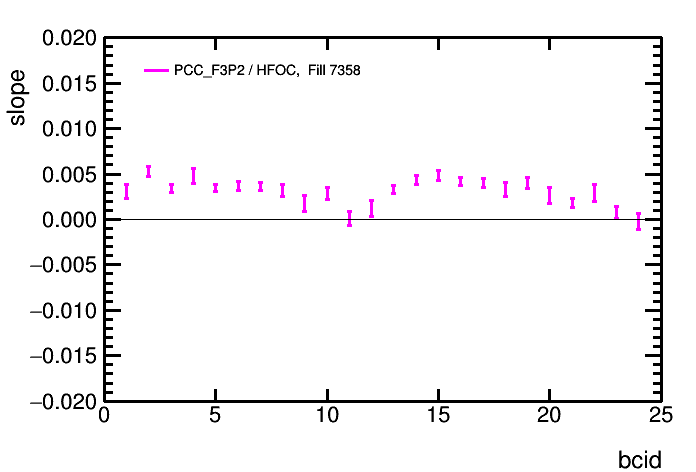
\includegraphics[width=0.32\linewidth]{plots/sbilratios_trains_Fill7358/plot_det_linearity_perbx_slope_7358_F3p2.png}
    \caption{
      Slope values obtained from the linearity fits for the 24 bunches in the two trains of Fill 7358.
      In this plots PCC is shown separately for: \\
      {\bf BPIX} layer 1 (top-left), layer 2 (top-middle), layer 3 (top-right) , \\
      {\bf FPIX Panel 1}:  disk 1 (middle-left), disk 2 (middle-middle), disk 3 (middle-right), and \\
      {\bf FPIX Panel 2}: disk 1 (bottom-left), disk 2 (bottom-middle), disk 3 (bottom-right).
      \label{fig:fill7358trainslope_pccparts}
    }
  \end{center}
\end{figure}

\clearpage
\newpage
\section{Summary}
In this note the relative linearity between PCC and other luminometers has been studied using special runs recorded in 2018 which included pile-up scans up to 100.
The linearity is determined by fitting the ratio of two luminometers as a funcion of SBIL measured by a reference detector, in this case the HFOC has been chosen as reference.
Isolated, leading, and train bunches are used to study the variations and train or afterglow effects.

Using isolated and leading bunches a slope of $0.32\pm0.04 \% [Hz/\mu b]^{-1}$ is obtained for the PCC/HFOC comparison.
For train bunches in fill 7358 a systematic decrease is observed in the slope as a function of the bunch id, where the slope becomes negative after 12 bunches.
This effect has been studied by removing the afterglow corrections for PCC and HFOC and by dividing the PCC into subdetectors.
This effect indicates the PCC suffers a loss in cluster counts possibly due to high occupancies at high pileup. 
A variation of the effect is observed for different parts of the Pixel detector.



% >> acknowledgments (for journal papers only)
% The latest version of the acknowledgments will be included from https://twiki.cern.ch/twiki/bin/viewauth/CMS/Internal/PubAcknow as of the date of submission. Modify to match either US or UK English spelling for centre/center, programme/program. For PRL use the short version, for JINST normally use the long version. All others take the middle length version other than exceptional cases.
%\begin{acknowledgments}
%\end{acknowledgments}

%% **DO NOT REMOVE BIBLIOGRAPHY**
\bibliography{auto_generated}   % will be created by the tdr script.

%% examples of appendices.
\clearpage
\appendix
\section{Pixel module veto list}
\label{sec:appendix1}

List of Pixel module id's used to remove modules with unstable behavior. Version used for the PCC luminosity of second half of 2018 Run D. 

{
\tiny
%\begin{multicols}{10}
 303042564
 303042568
 303042572
 303042576
 303042580
 303042588
 303042592
 303046660
 303046664
 303046668
 303046672
 303046676
 303046680
 303046684
 303046688
 303050760
 303050764
 303050768
 303050772
 303050776
 303050780
 303050784
 303054852
 303054856
 303054860
 303054864
 303054868
 303054872
 303054876
 303054880
 303058948
 303058952
 303058956
 303058960
 303058964
 303058968
 303058972
 303058976
 303063044
 303063048
 303063052
 303063056
 303063060
 303063064
 303063068
 303063072
 303067140
 303067144
 303067148
 303067152
 303067156
 303067160
 303067164
 303067168
 303071236
 303071240
 303071244
 303071248
 303071252
 303071256
 303071260
 303071264
 303075332
 303075336
 303075340
 303075344
 303075348
 303075352
 303075356
 303075360
 303079428
 303079432
 303079436
 303079440
 303079444
 303079448
 303079452
 303079456
 303083524
 303083528
 303083532
 303083536
 303083540
 303083544
 303083548
 303083552
 303087620
 303087624
 303087628
 303087632
 303087636
 303087640
 303087644
 303087648
 304091140
 304091144
 304091148
 304091156
 304091160
 304091164
 304091168
 304095236
 304095240
 304095244
 304095248
 304095252
 304095256
 304095260
 304095264
 304099332
 304099336
 304099340
 304099344
 304099348
 304099352
 304099356
 304099360
 304103428
 304103432
 304103436
 304103440
 304103444
 304103448
 304103452
 304103456
 304107524
 304107528
 304107532
 304107536
 304107540
 304107544
 304107548
 304111620
 304111624
 304111628
 304111632
 304111636
 304111640
 304111644
 304111648
 304115716
 304115720
 304115724
 304115728
 304115732
 304115736
 304115740
 304115744
 304119812
 304119816
 304119820
 304119824
 304119828
 304119832
 304119836
 304119840
 304123908
 304123912
 304123916
 304123924
 304123928
 304123932
 304123936
 304128004
 304128008
 304128012
 304128016
 304128020
 304128024
 304128028
 304128032
 304132100
 304132104
 304132108
 304132112
 304132116
 304132120
 304132124
 304132128
 304136196
 304136200
 304136204
 304136212
 304136216
 304136220
 304136224
 304140292
 304140296
 304140300
 304140304
 304140308
 304140312
 304140316
 304140320
 304144388
 304144392
 304144396
 304144400
 304144404
 304144408
 304144412
 304144416
 304148484
 304148488
 304148492
 304148496
 304148500
 304148504
 304148508
 304148512
 304152580
 304152584
 304152588
 304152592
 304152596
 304152600
 304152604
 304152608
 304156676
 304156680
 304156684
 304156688
 304156692
 304156696
 304156700
 304156704
 304160772
 304160776
 304160780
 304160784
 304160788
 304160792
 304160796
 304160800
 304164868
 304164872
 304164876
 304164880
 304164884
 304164888
 304164892
 304164896
 304168964
 304168968
 304168972
 304168984
 304168988
 304168992
 304173060
 304173064
 304173068
 304173072
 304173076
 304173080
 304173084
 304173088
 304177156
 304177160
 304177164
 304177168
 304177172
 304177176
 304177180
 304177184
 304181252
 304181256
 304181260
 304181264
 304181268
 304181272
 304181276
 304181280
 304185348
 304185352
 304185356
 304185360
 304185364
 304185368
 304185372
 304185376
 304189444
 304189448
 304189452
 304189456
 304189460
 304189464
 304189468
 304189472
 304193540
 304193544
 304193548
 304193552
 304193556
 304193560
 304193564
 304193568
 304197636
 304197640
 304197644
 304197648
 304197652
 304197656
 304197660
 304197664
 304201732
 304201736
 304201740
 304201744
 304201748
 304201752
 304201756
 304201760
 305139728
 305139732
 305139736
 305139740
 305139744
 305143812
 305143816
 305143820
 305143824
 305143828
 305143832
 305143836
 305143840
 305147912
 305147916
 305147924
 305147928
 305147932
 305147936
 305152008
 305152012
 305152020
 305152024
 305152028
 305152032
 305156104
 305156116
 305156120
 305156124
 305156128
 305160200
 305160212
 305160216
 305160220
 305160224
 305164308
 305164312
 305164316
 305164320
 305168392
 305168396
 305168400
 305168404
 305168408
 305168412
 305168416
 305172492
 305172500
 305172504
 305172508
 305172512
 305176580
 305176596
 305176600
 305176604
 305176608
 305180676
 305180688
 305180692
 305180696
 305180700
 305180704
 305184784
 305184788
 305184792
 305184796
 305184800
 305188868
 305188872
 305188876
 305188884
 305188888
 305188892
 305188896
 305192964
 305192972
 305192976
 305192980
 305192984
 305192988
 305192992
 305197060
 305197068
 305197076
 305197080
 305197084
 305197088
 305201156
 305201160
 305201164
 305201168
 305201172
 305201176
 305201180
 305201184
 305205252
 305205256
 305205264
 305205268
 305205272
 305205276
 305205280
 305209348
 305209352
 305209356
 305209364
 305209368
 305209372
 305209376
 305213444
 305213452
 305213460
 305213464
 305213468
 305213472
 305217540
 305217544
 305217548
 305217552
 305217556
 305217560
 305217564
 305217568
 305221636
 305221640
 305221652
 305221656
 305221660
 305221664
 305225736
 305225740
 305225748
 305225752
 305225756
 305225760
 305229828
 305229832
 305229836
 305229840
 305229844
 305229848
 305229852
 305229856
 305233924
 305233932
 305233936
 305233940
 305233944
 305233948
 305233952
 305238028
 305238032
 305238036
 305238040
 305238044
 305238048
 305242120
 305242132
 305242136
 305242140
 305242144
 305246224
 305246232
 305246236
 305246240
 305250308
 305250324
 305250328
 305250332
 305250336
 305254416
 305254420
 305254424
 305254432
 305258500
 305258504
 305258508
 305258512
 305258516
 305258520
 305258524
 305258528
 305262596
 305262604
 305262608
 305262612
 305262616
 305262620
 305266696
 305266708
 305266712
 305266716
 305266720
 305270788
 305270792
 305270796
 305270804
 305270808
 305270812
 305270816
 305274884
 305274892
 305274900
 305274904
 305274908
 305274912
 305278988
 305278992
 305278996
 305279000
 305279004
 305279008
 305283076
 305283080
 305283092
 305283096
 305283100
 305287172
 305287180
 305287192
 305287196
 305291268
 305291272
 305291276
 305291280
 305291284
 305291288
 305291292
 305291296
 305295364
 305295368
 305295376
 305295380
 305295384
 305295388
 305295392
 305299468
 305299476
 305299480
 305299484
 305303560
 305303576
 305303580
 305303584
 305307652
 305307656
 305307660
 305307668
 305307672
 305307676
 305307680
 305311748
 305311764
 305311768
 305311772
 305311776
 305315852
 305315856
 305315860
 305315864
 305315868
 305315872
 306188296
 306188312
 306188316
 306188320
 306192388
 306192400
 306192404
 306192408
 306192412
 306192416
 306196500
 306196504
 306196508
 306196512
 306200584
 306200596
 306200604
 306200608
 306204684
 306204692
 306204696
 306204700
 306204704
 306208788
 306208792
 306208796
 306208800
 306212868
 306212872
 306212876
 306212880
 306212884
 306212888
 306212892
 306212896
 306216964
 306216972
 306216980
 306216984
 306216988
 306216992
 306221064
 306221068
 306221072
 306221076
 306221084
 306221088
 306225160
 306225164
 306225172
 306225176
 306225180
 306225184
 306229260
 306229264
 306229268
 306229272
 306229280
 306233352
 306233360
 306233364
 306233368
 306233376
 306237448
 306237452
 306237456
 306237460
 306237464
 306237468
 306237472
 306241544
 306241548
 306241556
 306241560
 306241564
 306241568
 306245636
 306245644
 306245648
 306245652
 306245656
 306245660
 306245664
 306249732
 306249736
 306249740
 306249748
 306249752
 306249756
 306249760
 306253844
 306253856
 306257936
 306257944
 306257948
 306257952
 306262024
 306262028
 306262048
 306266124
 306266128
 306266132
 306266136
 306266140
 306270212
 306270228
 306270232
 306270240
 306274332
 306278420
 306278424
 306278432
 306282508
 306282520
 306282524
 306282528
 306286596
 306286604
 306286616
 306286624
 306290692
 306290700
 306290704
 306294804
 306294808
 306294812
 306298900
 306298904
 306298908
 306298912
 306302980
 306302984
 306302988
 306302996
 306303004
 306303008
 306307088
 306307096
 306311172
 306311184
 306311200
 306315268
 306315272
 306315288
 306319368
 306319372
 306319376
 306319380
 306319384
 306319388
 306319392
 306323468
 306323484
 306323488
 306327560
 306327572
 306327576
 306327584
 306331652
 306331656
 306331664
 306331668
 306331672
 306335748
 306335756
 306335760
 306335764
 306335768
 306335772
 306335776
 306339844
 306339860
 306339868
 306339872
 306343940
 306343944
 306343956
 306343964
 306343968
 306348036
 306348040
 306348056
 306348060
 306352132
 306352136
 306352140
 306352148
 306352152
 306352156
 306352160
 306356232
 306356244
 306356248
 306356252
 306360332
 306360344
 306360348
 306364436
 306364440
 306364448
 306368532
 306368536
 306368544
 306372612
 306372640
 306376708
 306376712
 306376728
 306376732
 306380804
 306380812
 306380820
 306384904
 306384920
 306384924
 306384928
 306388996
 306389004
 306389016
 306389020
 306393092
 306393108
 306393112
 306393116
 306393120
 306397188
 306397192
 306397196
 306397200
 306397204
 306397208
 306397216
 306401284
 306401288
 306401296
 306401300
 306401304
 306401308
 306401312
 306405384
 306405392
 306405396
 306405400
 306405404
 306409480
 306409484
 306409496
 306409500
 306409504
 306413572
 306413580
 306413592
 306413596
 306417672
 306417676
 306417680
 306417684
 306417688
 306417692
 306417696
 306421764
 306421780
 306421784
 306421788
 306421792
 306425860
 306425864
 306425868
 306425880
 306425884
 306425888
 306429956
 306429960
 306429964
 306429968
 306429972
 306429976
 306429980
 306429984
 306434052
 306434068
 306434072
 306434076
 306434080
 306438148
 306438156
 306438160
 306442252
 306442260
 306442264
 306442268
 306442272
 306446340
 306446356
 306446360
 306446364
 306446368
 344201220
 344204292
 344205316
 344208388
 344209412
 344212484
 344213508
 344216580
 344217604
 344220676
 344221700
 344225796
 344229892
 344233988
 344238084
 344241156
 344242180
 344246276
 344249348
 344250372
 344253444
 344254468
 344257540
 344258564
 344261636
 344262660
 344265732
 344266756
 344269828
 344270852
 344274948
 344278020
 344279044
 344282116
 344283140
 344291332
 344294404
 344295428
 344298500
 344299524
 344302596
 344303620
 344307716
 344310788
 344311812
 344314884
 344315908
 344318980
 344320004
 344323076
 344324100
 344328196
 344332292
 344335364
 344336388
 344339460
 344340484
 344344580
 344348676
 344355844
 344359940
 344360964
 344365060
 344369156
 344372228
 344373252
 344376324
 344377348
 344380420
 344384516
 344385540
 344388612
 344389636
 344393732
 344396804
 344397828
 344401924
 344404996
 344406020
 344409092
 344410116
 344413188
 344417284
 344418308
 344422404
 344425476
 344426500
 344462340
 344463364
 344466436
 344467460
 344470532
 344471556
 344474628
 344475652
 344478724
 344479748
 344482820
 344483844
 344486916
 344487940
 344492036
 344495108
 344496132
 344499204
 344500228
 344504324
 344508420
 344511492
 344512516
 344515588
 344516612
 344519684
 344520708
 344523780
 344524804
 344528900
 344532996
 344536068
 344537092
 344540164
 344541188
 344544260
 344545284
 344548356
 344549380
 344552452
 344553476
 344556548
 344560644
 344561668
 344568836
 344569860
 344572932
 344573956
 344577028
 344578052
 344581124
 344582148
 344585220
 344586244
 344589316
 344597508
 344598532
 344602628
 344605700
 344606724
 344609796
 344610820
 344613892
 344614916
 344617988
 344626180
 344627204
 344630276
 344631300
 344638468
 344642564
 344646660
 344647684
 344650756
 344651780
 344658948
 344659972
 344663044
 344664068
 344667140
 344668164
 344671236
 344672260
 344676356
 344679428
 344680452
 344684548
 344687620
 344688644
 344725508
 344729604
 344733700
 344736772
 344740868
 344741892
 344744964
 344745988
 344749060
 344750084
 344753156
 344754180
 344757252
 344758276
 344761348
 344762372
 344765444
 344766468
 344769540
 344770564
 344774660
 344777732
 344778756
 344781828
 344782852
 344785924
 344786948
 344790020
 344791044
 344794116
 344795140
 344798212
 344799236
 344802308
 344803332
 344806404
 344807428
 344811524
 344814596
 344818692
 344822788
 344823812
 344826884
 344827908
 344830980
 344835076
 344836100
 344843268
 344844292
 344847364
 344848388
 344851460
 344852484
 344855556
 344859652
 344860676
 344863748
 344864772
 344867844
 344868868
 344871940
 344872964
 344876036
 344877060
 344881156
 344884228
 344889348
 344892420
 344896516
 344900612
 344901636
 344904708
 344908804
 344909828
 344913924
 344921092
 344922116
 344925188
 344929284
 344930308
 344933380
 344937476
 344938500
 344942596
 344946692
 344950788
 352588804
 352589828
 352592900
 352593924
 352596996
 352601092
 352602116
 352605188
 352606212
 352609284
 352610308
 352613380
 352617476
 352618500
 352621572
 352622596
 352625668
 352626692
 352629764
 352630788
 352633860
 352634884
 352637956
 352638980
 352642052
 352643076
 352646148
 352647172
 352651268
 352654340
 352655364
 352658436
 352659460
 352662532
 352663556
 352666628
 352667652
 352670724
 352671748
 352675844
 352678916
 352679940
 352683012
 352684036
 352687108
 352688132
 352691204
 352692228
 352695300
 352696324
 352699396
 352700420
 352703492
 352704516
 352707588
 352708612
 352711684
 352712708
 352715780
 352719876
 352720900
 352724996
 352737284
 352740356
 352741380
 352744452
 352745476
 352748548
 352749572
 352753668
 352756740
 352757764
 352761860
 352764932
 352765956
 352770052
 352774148
 352781316
 352782340
 352786436
 352789508
 352790532
 352793604
 352794628
 352797700
 352798724
 352801796
 352802820
 352805892
 352806916
 352809988
 352811012
 352814084
 352815108
 352850948
 352851972
 352855044
 352856068
 352859140
 352860164
 352863236
 352864260
 352868356
 352871428
 352872452
 352875524
 352876548
 352879620
 352880644
 352883716
 352884740
 352888836
 352892932
 352896004
 352897028
 352900100
 352901124
 352904196
 352905220
 352908292
 352909316
 352912388
 352913412
 352917508
 352920580
 352921604
 352924676
 352925700
 352928772
 352929796
 352933892
 352936964
 352937988
 352941060
 352945156
 352949252
 352950276
 352953348
 352954372
 352957444
 352958468
 352962564
 352965636
 352966660
 352973828
 352974852
 352982020
 352987140
 352990212
 352995332
 352999428
 353002500
 353006596
 353010692
 353015812
 353018884
 353019908
 353022980
 353024004
 353028100
 353032196
 353044484
 353047556
 353048580
 353052676
 353060868
 353063940
 353064964
 353068036
 353069060
 353073156
 353076228
 353114116
 353118212
 353122308
 353125380
 353126404
 353129476
 353130500
 353133572
 353134596
 353137668
 353138692
 353141764
 353142788
 353145860
 353146884
 353149956
 353150980
 353154052
 353155076
 353158148
 353159172
 353162244
 353163268
 353166340
 353167364
 353170436
 353174532
 353175556
 353178628
 353179652
 353183748
 353187844
 353190916
 353191940
 353195012
 353196036
 353199108
 353200132
 353203204
 353204228
 353207300
 353208324
 353211396
 353212420
 353215492
 353216516
 353219588
 353223684
 353224708
 353228804
 353231876
 353235972
 353240068
 353244164
 353248260
 353249284
 353252356
 353256452
 353261572
 353268740
 353281028
 353282052
 353285124
 353286148
 353290244
 353293316
 353298436
 353302532
 353305604
 353309700
 353313796
 353314820
 353317892
 353321988
 353323012
 353326084
 353327108
 353330180
 353331204
 353334276
 353338372
 353339396
%\end{multicols}

}

\section{Train effect crosscheck}
\label{sec:appendix2}

Two cross-checks have been performed for Fill 7358 to understand if the systematic change in the slope values as a function of bcid are due to the afterglow corrections.
In the first check (Fig~\ref{fig:fill7358trainslope_crosscheckPCC}) the PCC afterglow corrections are removed, in the second check (Fig~\ref{fig:fill7358trainslope_crosscheckHFOC}) the HFOC residual afterglow corrections are removed.
In both tests the y-intercept values change, but the systematic trend on the slope values remains.

\vspace{36pt}
\begin{figure}[hc]
  \begin{center}
    \includegraphics[width=0.47\linewidth]{plots/sbilratios_trains_Fill7358/plot_det_linearity_perbx_y0_7358_NoPCCCorr.png}
    \includegraphics[width=0.47\linewidth]{plots/sbilratios_trains_Fill7358/plot_det_linearity_perbx_slope_7358_NoPCCCorr.png}
    \caption{
      y-intercept and slope values obtained from the linearity fits for the 24 bunches in the two trains of Fill 7358 after removing the PCC afterglow corrections.
      \label{fig:fill7358trainslope_crosscheckPCC}
    }

    \includegraphics[width=0.47\linewidth]{plots/sbilratios_trains_Fill7358/plot_det_linearity_perbx_y0_7358_NoHFCorr.png}
    \includegraphics[width=0.47\linewidth]{plots/sbilratios_trains_Fill7358/plot_det_linearity_perbx_slope_7358_NoHFCorr.png}
    \caption{
      y-intercept and slope values obtained from the linearity fits for the 24 bunches in the two trains of Fill 7358 after removing the HFOC residual afterglow corrections.
      \label{fig:fill7358trainslope_crosscheckHFOC}
    }

  \end{center}
\end{figure}


%\begin{figure}[hb]
%  \begin{center}
%  \end{center}
%\end{figure}
%


%%% DO NOT ADD \end{document}!

